\documentclass[12pt,parskip=full]{article}
\usepackage{lmodern}
\usepackage{amsmath}
\usepackage[left=1.0in,right=1.0in,top=0.5in,bottom=1.0in]{geometry}
\geometry{letterpaper}
\usepackage{graphicx}
\usepackage{caption}
\usepackage{subcaption}
\usepackage{longtable}
\usepackage{float}
\usepackage{wrapfig}
\usepackage{soul}
\usepackage{textcomp}
\usepackage{marvosym}
\usepackage{wasysym}
\usepackage{latexsym}
\usepackage{amssymb}
\usepackage{apacite}
\usepackage{tabu}
\usepackage[svgnames]{xcolor}
\usepackage{tikz}
\usepackage[linktoc=all]{hyperref}
\usepackage{cleveref}
\usepackage{listings}
\usepackage{setspace}
\usepackage{parskip}
\usepackage{array}
\usepackage{apacite}
\usepackage{natbib}
\usepackage{multicol}
\usepackage{subcaption}
\usepackage{mathtools}
\usetikzlibrary{arrows}

\pgfdeclarelayer{edgelayer}
\pgfdeclarelayer{nodelayer}
\pgfsetlayers{edgelayer,nodelayer,main}

\tikzstyle{none}=[inner sep=0pt]
\tikzstyle{waypt}=[circle,fill=Black,draw=Black,scale=0.4]
\tikzstyle{Helobody}=[circle,fill=White,draw=Black,scale=4.0]
\tikzstyle{Tailrotor}=[circle,fill=White,draw=Black,scale=1.0]
\tikzstyle{ForceVector}=[->,draw=Indigo,fill=Indigo]
\tikzstyle{Coordinate}=[->,draw=Red,fill=Red,fill opacity=1.0]
\tikzstyle{angle}=[->]
\tikzstyle{MeasureMark}=[|-|]
\newlength{\imagewidth}
\newlength{\imagescale}

\setlength{\parskip}{11pt}
%\setlength{\parindent}{15pt}
\usepackage{bookmark}
\makeatletter
%\renewcommand\@seccntformat[1]{}
\makeatother

\lstset
{
	language=c,
	keywords={break,case,catch,continue,else,for,
		if,return,switch,try,while,int,void},
	basicstyle=\ttfamily,
	keywordstyle=\color{blue},
	commentstyle=\color{ForestGreen},
	stringstyle=\color{purple},
	numbers=left,
	numberstyle=\tiny\color{gray},
	stepnumber=1,
	numbersep=10pt,
	backgroundcolor=\color{white},
	tabsize=4,
	showspaces=false,
	showstringspaces=false
}

\renewcommand{\thesection}{\arabic{section}}

\renewcommand{\thesubsection}{\thesection\alph{subsection}}
\renewcommand{\theequation}{\thesubsection\arabic{equation}}
\newcommand*\circled[1]{\tikz[baseline=(char.base)]{
			\node[shape=circle,draw,inner sep=1pt] (char) {#1};}}
			
\numberwithin{subsection}{section}

\begin{document}
	\vspace{-4ex}
	\title{EbbCFD Theory Guide Part 2\vspace{-3.5ex}}
	\author{Rob Rau\vspace{-4ex}}
	\date{\today\vspace{-4ex}}
	\maketitle

	\section{Introduction}
		The last three months of work on EbbCFD have focused on 3 primary goals: Improvements to the plotting system in order to
		better display higher order results, impliment viscous flux terms in order to compute the full comressible Navier-Stokes 
		equations, and finally to empiricaly demonstrate the accuracy and convergence rate of EbbCFD.

	\section{High Order Plotting}
		Previously, EbbCFD could only plot cell averaged values, throwing away any additional information used used by the solver.
		The current solver also uses cell centered solution gradients and edge mid-point solution values. With this information
		a better solution estimate can be displayed.
		
		To address this ebb-reconstruct was developed in order to generate higher order visualizations. To do this, ebb-reconstruct
		breaks up each $N$ edge cell into $2N$ triangles. The verticies used for these new triangles are the cell centroid, the edge
		mid-points and the actual cell verticies. It then uses the cell centered gradients to interpolate solution values to the new
		verticies. Edge mid-points and cell verticies have multiple values associated with them after this step so the final value is
		the average of all values associated with a point.

		\begin{figure}[H]
			\centering
			\begin{subfigure}{0.4\textwidth}
				\hspace*{-2cm}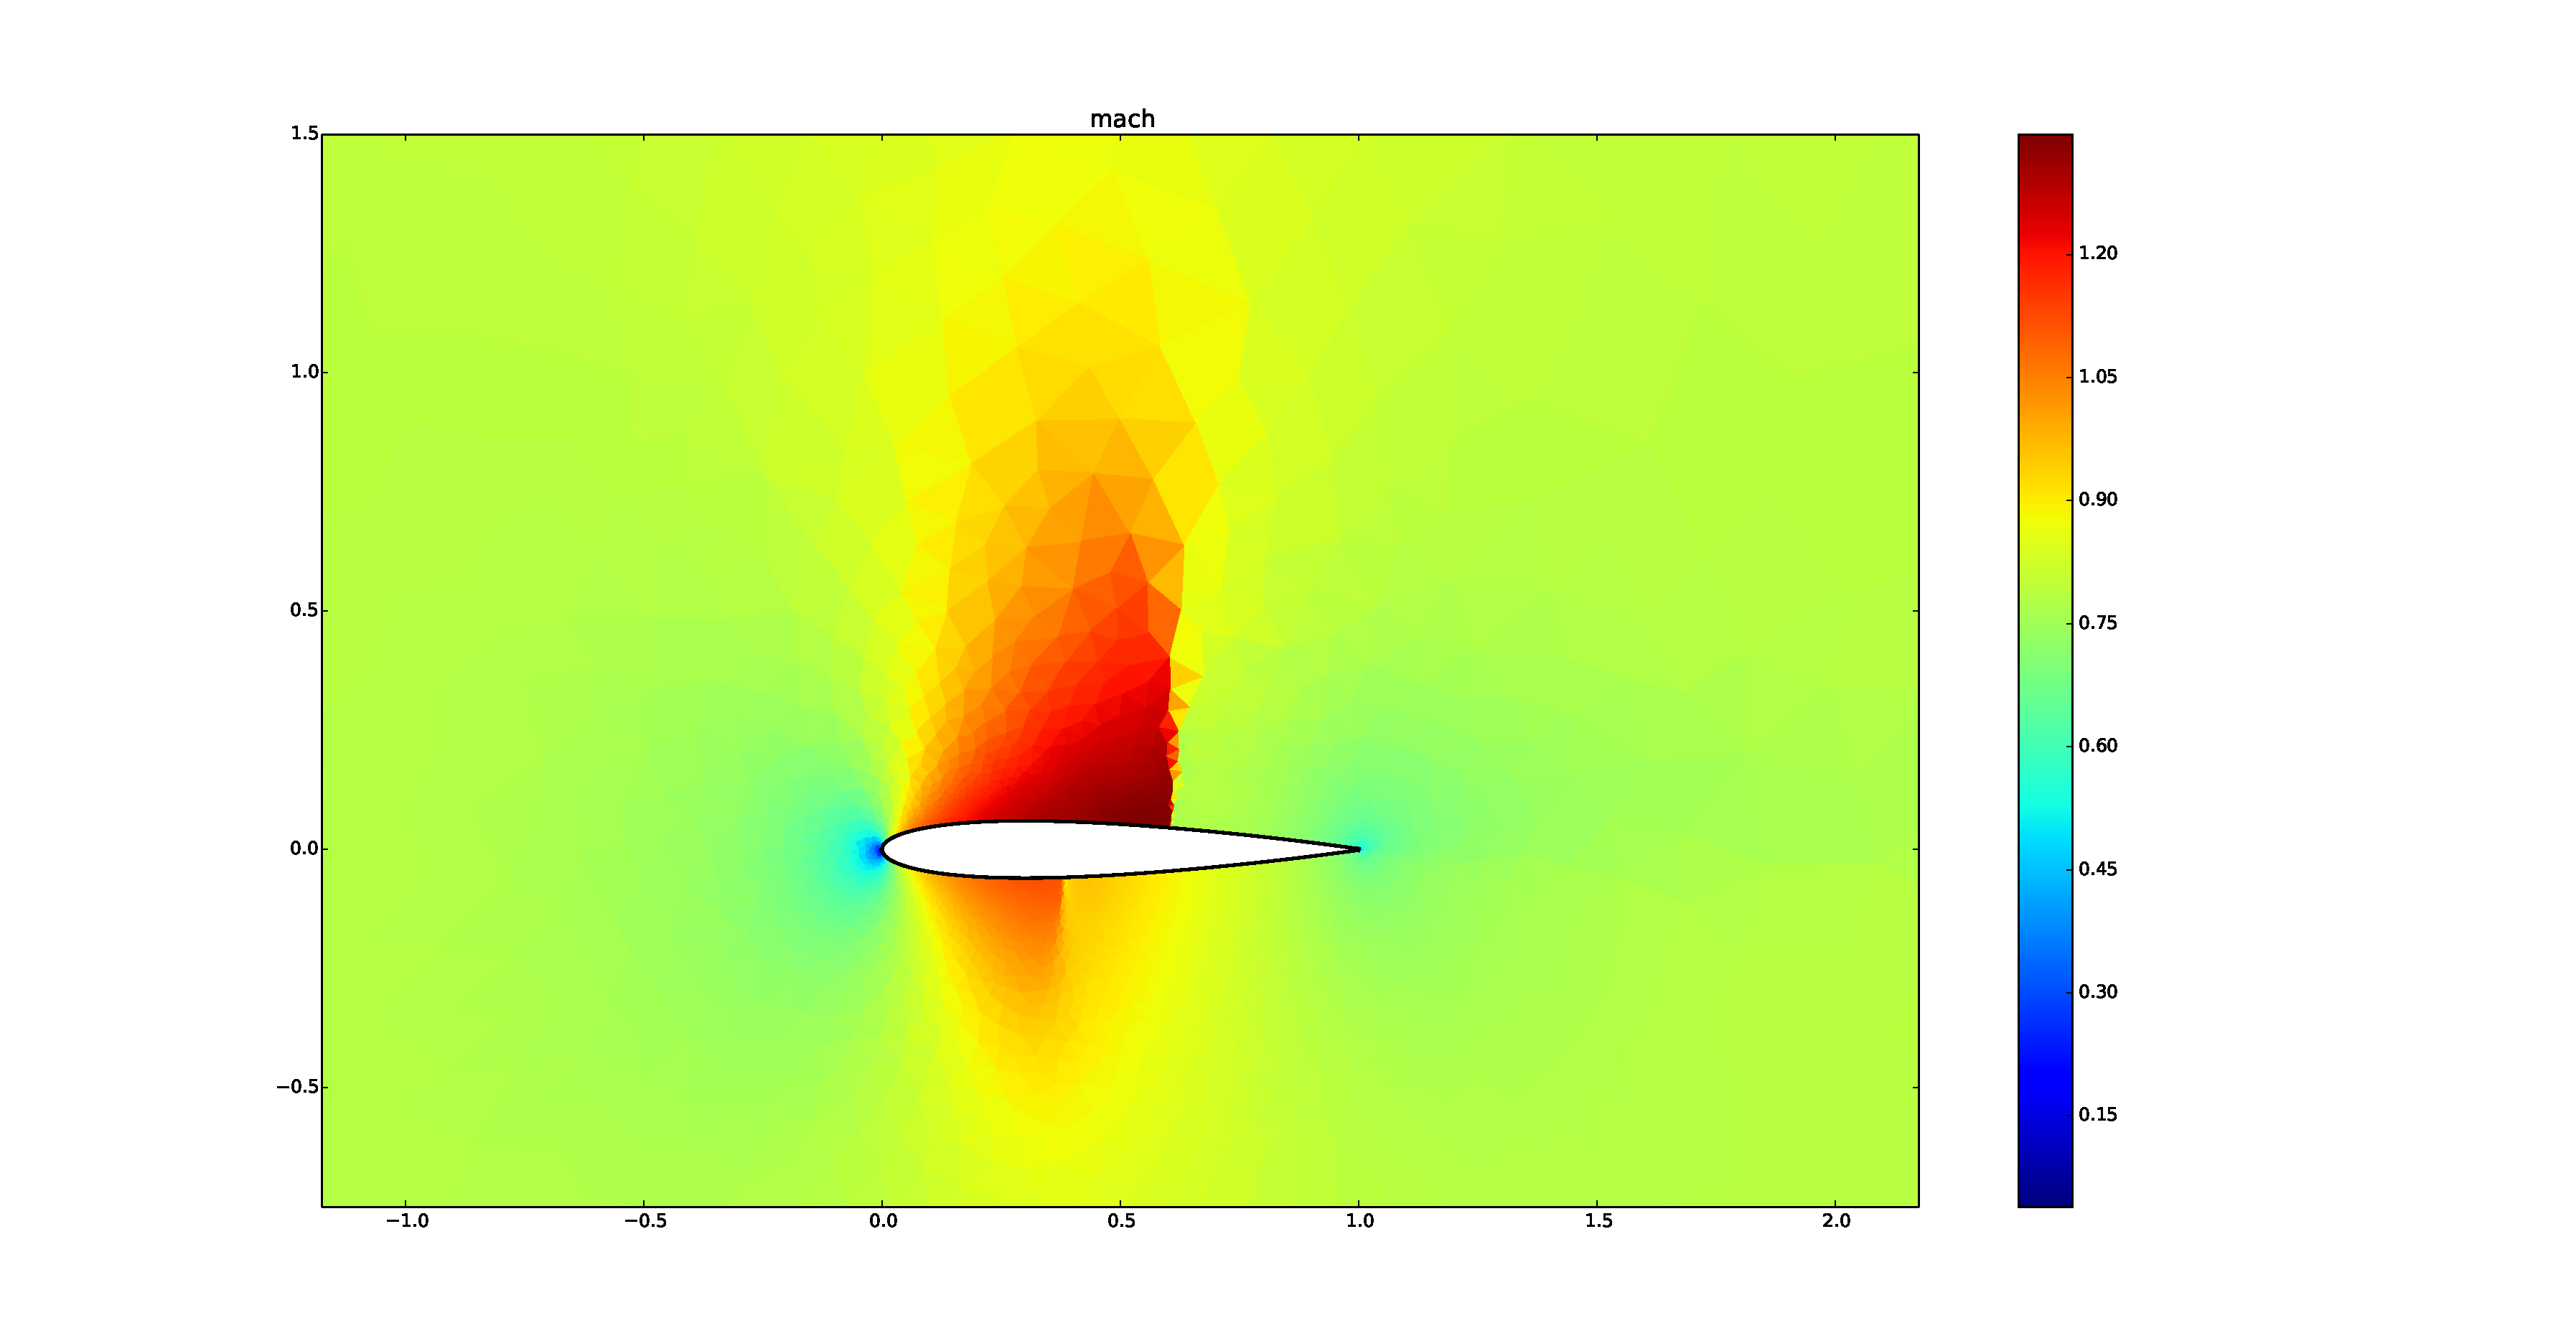
\includegraphics[scale=0.2,trim={7cm 2cm 10cm 2cm},clip]{CellAvgPlot.pdf}
				\hspace*{-2cm}\caption{Displaying only cell average values}
			\end{subfigure}
			\begin{subfigure}{0.4\textwidth}
				\hspace*{1cm}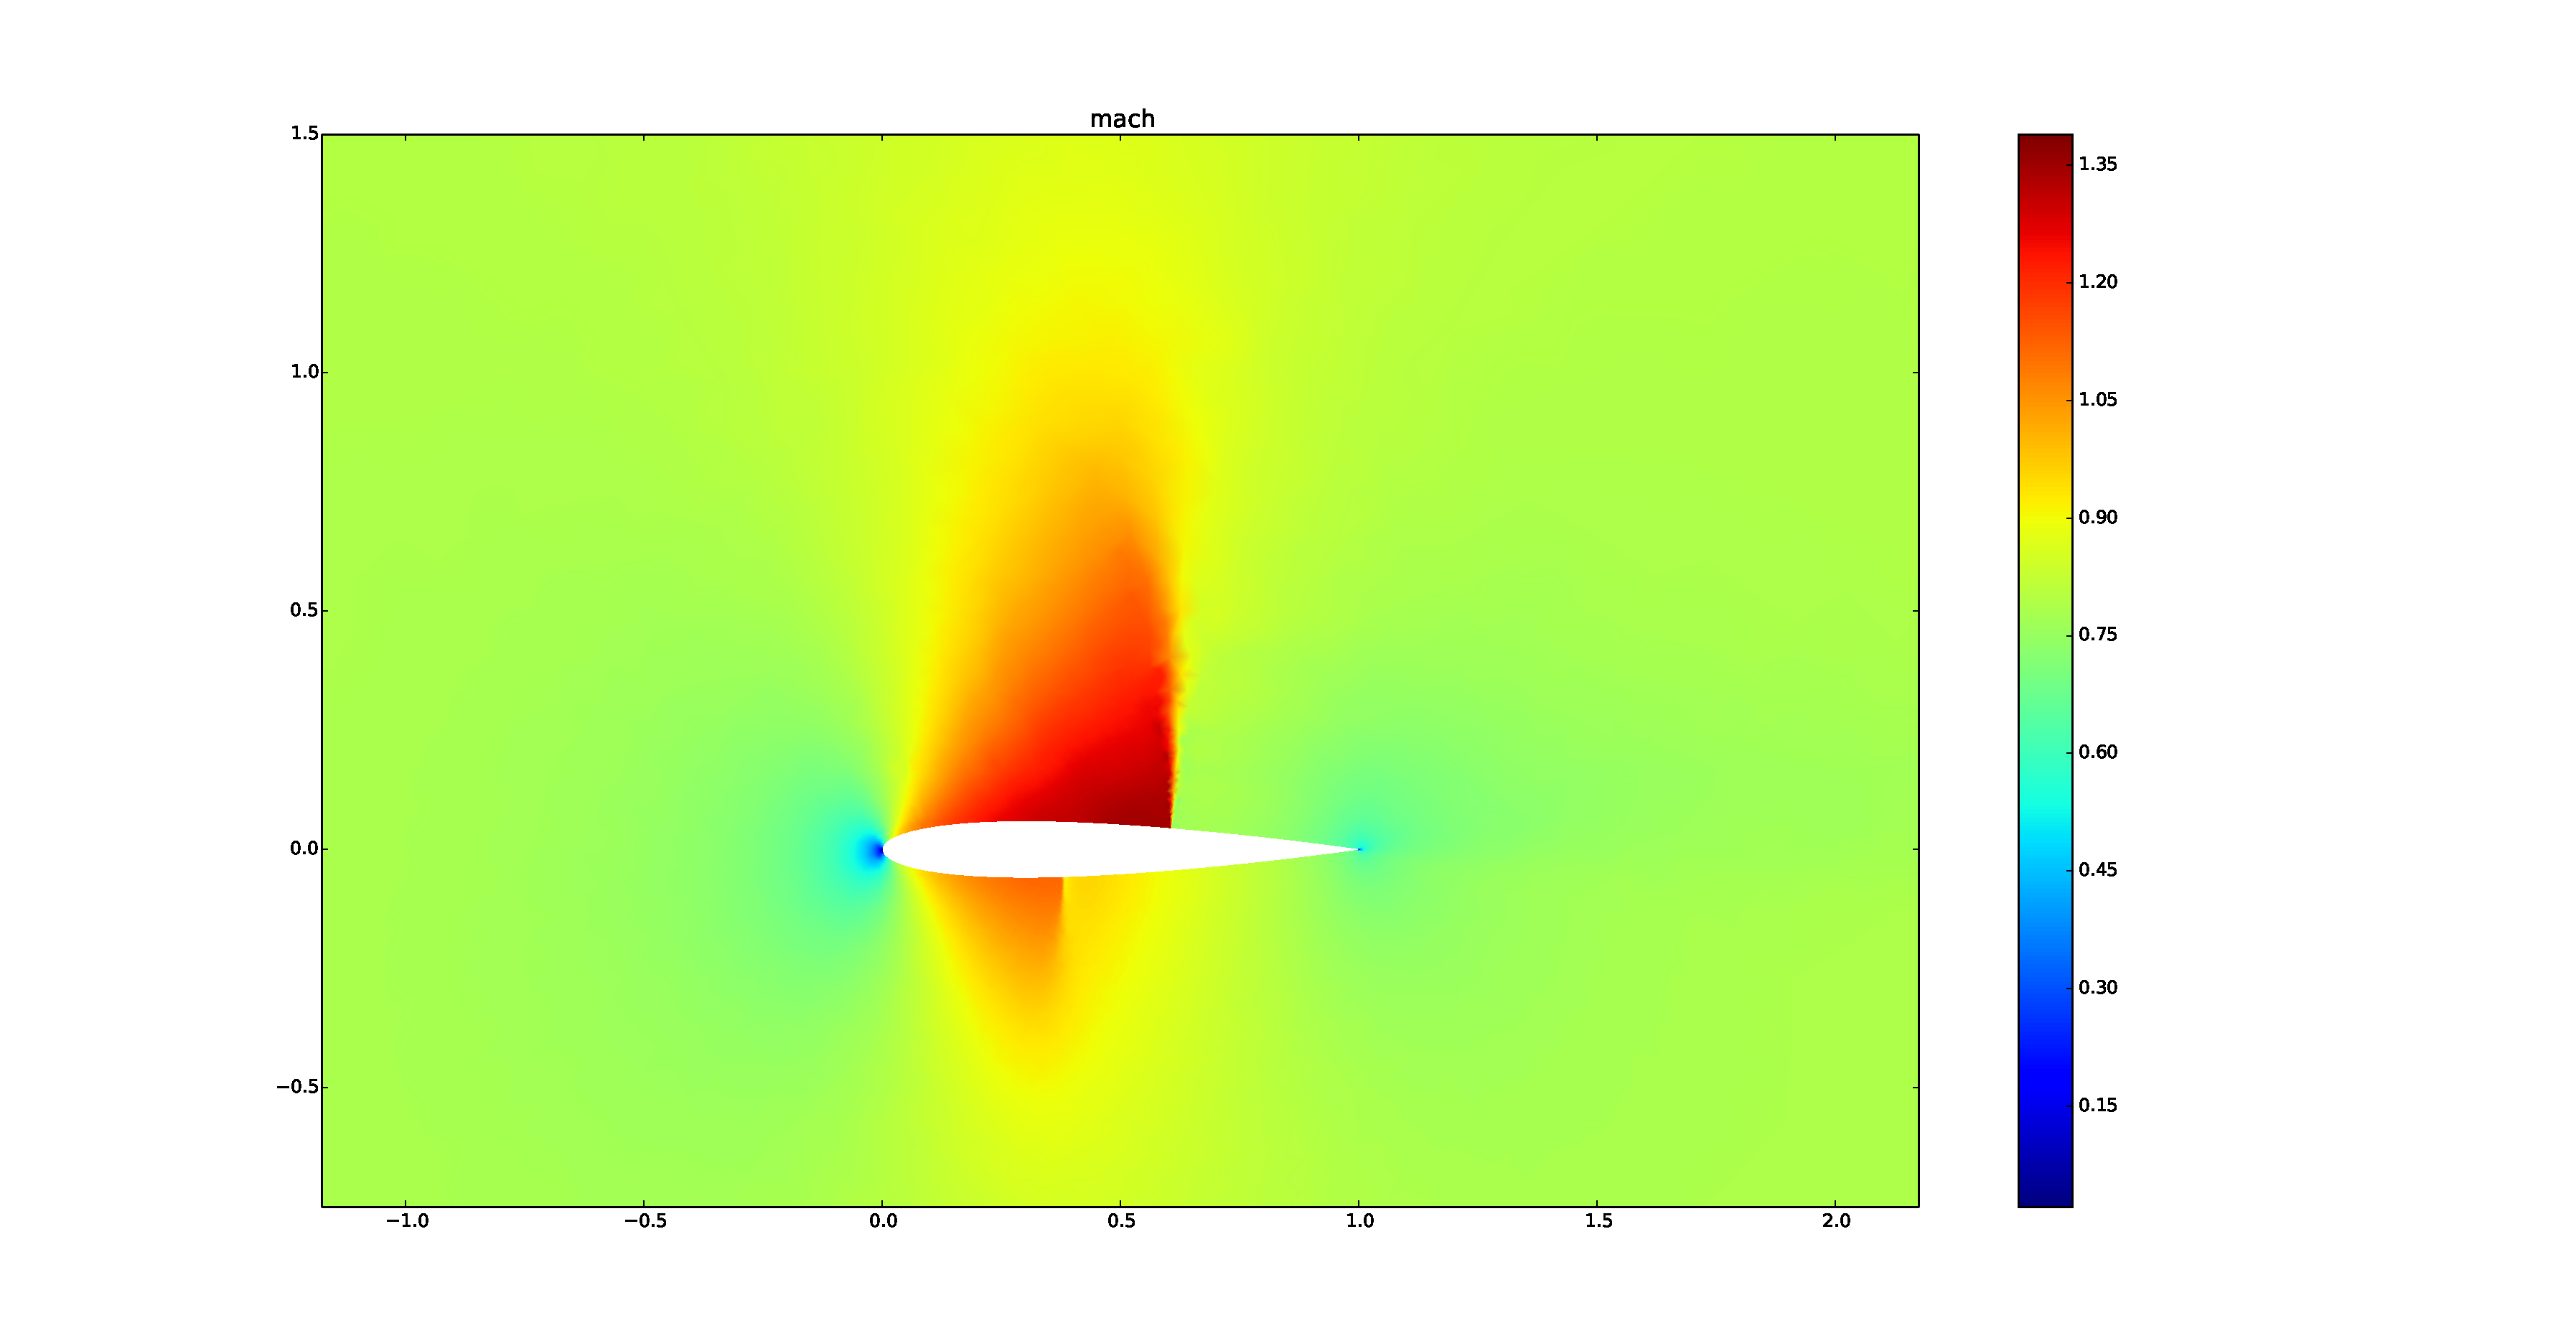
\includegraphics[scale=0.2,trim={7cm 2cm 10cm 2cm},clip]{ReconstructedPlot.pdf}
				\hspace*{1cm}\caption{Displaying reconstructed solution}
			\end{subfigure}
		\end{figure}
		
	\section{Navier-Stokes}
		The current Navier-Stokes implementation is a rather naive approach. It modifies the convective flux terms by adding a
		viscous flux term. The viscous term is computed as
		\begin{equation}
		\end{equation}
		This involves making a approximation of the solution gradient at the cell interface. EbbCFD currently does this by simply
		taking the average of the solution gradient of the neighboring cells.
		
		
		This provides a stable scheme at low Reynolds numbers, but does not show favorable convergence, as shown later. To address convergence I plan
		on implementing a version of the Bassi-Rebay 2 viscous discritization adapted for finite volumes.

		To show that the Navier-Stokes solution is accurate a flat plate simulation was performed and the drag results were compared to the
		Blassius solution.

		\begin{figure}[H]
			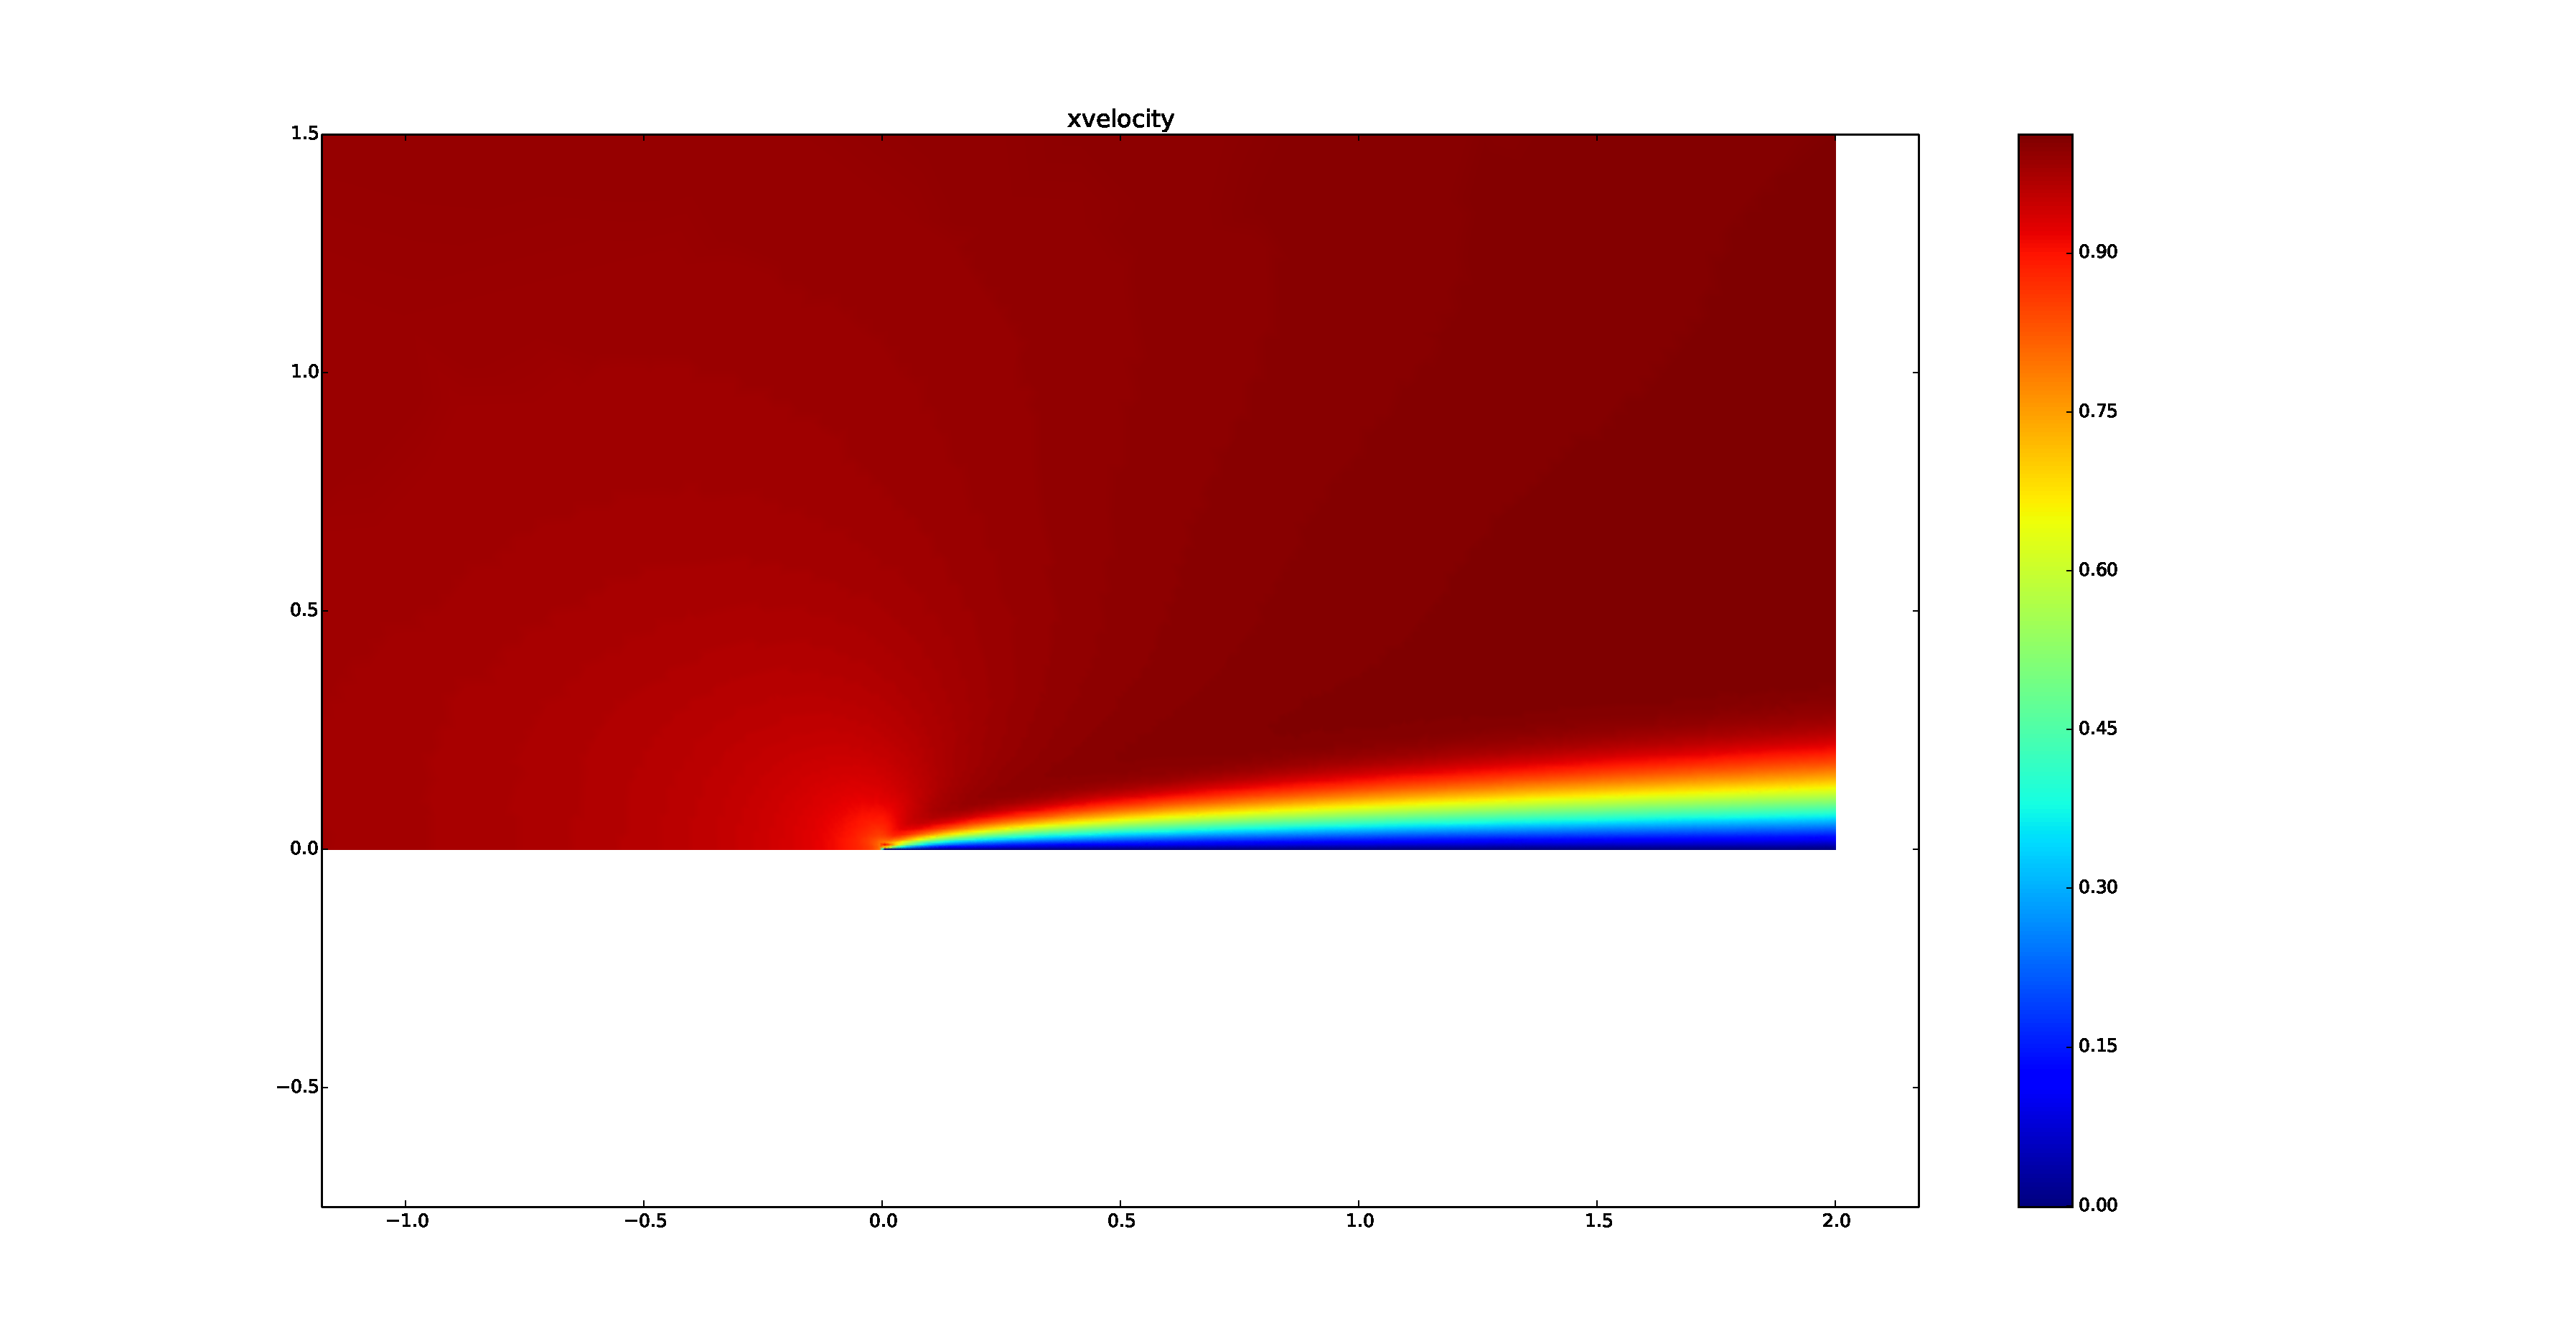
\includegraphics[width=\textwidth]{FlatPlate.pdf}
		\end{figure}
		
	\section{Method of Manufactured Solutions}
		To show that EbbCFD had correctly implimented its discritization, I employed the Method of Manufactured Solutions.
		The exact solution chosen was
		\begin{align}
			\rho &= a_\rho + b_\rho \sin(c_\rho x + d_\rho y) \\
			u &= a_u + b_u \cos(c_u x + d_u y) \\
			v &= a_v + b_v \cos(c_v x + d_v y) \\
			p &= a_p + b_p \sin(c_p x + d_p y)
		\end{align}

		\begin{figure}[H]
			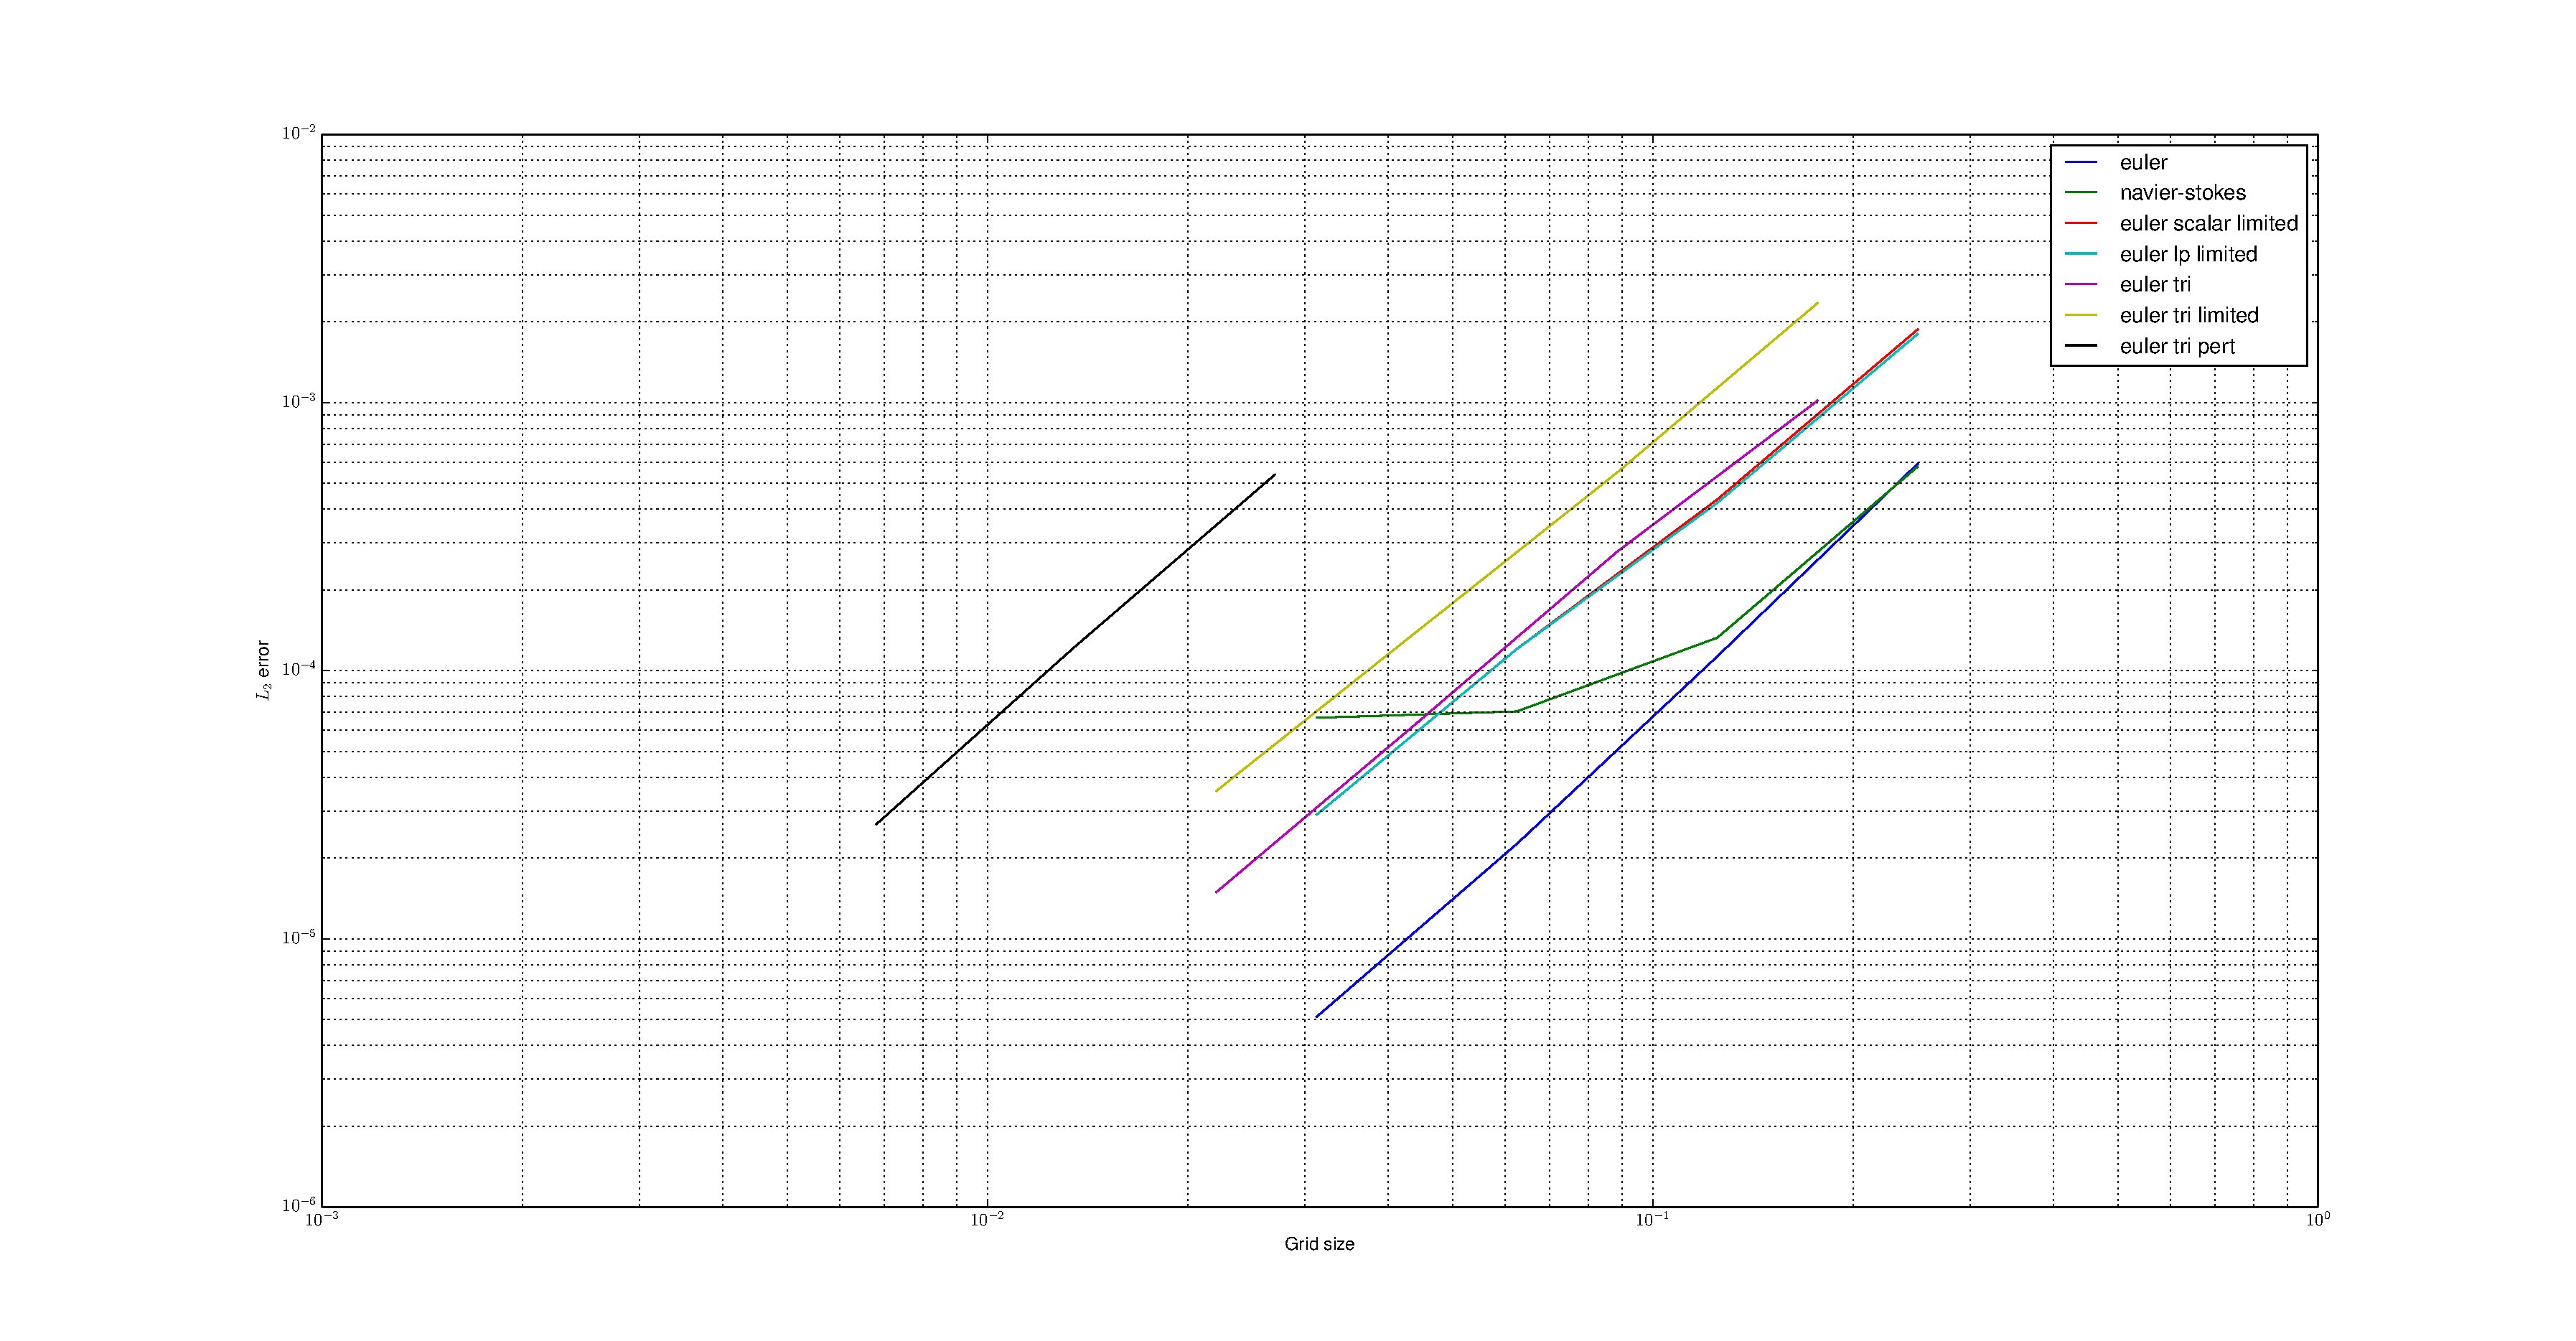
\includegraphics[width=\textwidth]{ConvergencePlot.pdf}
		\end{figure}
\end{document}
